\section{Overview}
\label{sec:overview}

In DockerGate, we propose to analyze the docker image by performing static analysis on the binaries shipped within the images. Using the results of the static analysis we identify the system calls used and generate a seccomp profile. When a docker image is executed as a container, on a seccomp enabled container, it loads a default profile, which allows the container to access almost all system calls on the host. This results in a large attack surface on the host kernel. 

In DockerGate, we analyze the docker image and identify the binary packages which can make various system calls to the host. Performing the analysis on docker images presents several implementation challenges:

\textit{Use of Dynamic Linked Libraries :} In modern practices, binary programs don’t perform a system call directly, instead they use libraries that are linked at runtime which act as wrapper functions to call the system calls. 

\textit{Analyzing libraries that link to other libraries:} Libraries are often dynamically linked to other libraries which in turn are linked to other libraries. Recursively going through each library cost too much time and we had to come up with a solution that required to cache this analysis

We identified a set of images suitable for testing from Docker Hub and analyzed the Dockerfiles for each image to determine the base image, and finalize on the data set. We used a web scraper to select random images from community image, similar to technique used by Shu et al~\cite{shu} in developing and downloading data set for their experiments. We used banyanops/collector~\cite{banyanops} framework to pull these images and execute DockerGate specific scripts within the container. Based on the intermediate results of the DockerGate scripts and a global database of system call mappings we generate a policy in json format, as specified in docker docs~\cite{seccomp}.

Figure \ref{fig:overview} shows major components of the DockerGate framework. An image name is provided to the DockerGate framework to generate the seccomp policy. In the first stage, the \textit{Analysis Engine} uses the banyanops collector framework’s ability to pull the docker image from Docker hub. The banyanops framework is configured to execute scripts to perform static analysis within the container. In this stage, banyanops iteratively creates a new containers of the docker image and execute the custom scripts to be executed within the container.
The intermediate output generated by these scripts is passed on to the \textit{Policy Generator} submodule to determine the system calls performed by the binaries within the container. 

In the Policy Generator, the intermediate output generated is checked for the library function calls it makes and it consults a predefined database of library functions. This database consists of records of standard glibc library~\cite{glibc}, pthread library functions. Each library function is associated with the system calls it can perform. Based on the library functions called we determine a set of system calls that can be performed by the container. 

The library function call database consists of the records for standard libraries. The framework also supports analysis of any unconventional libraries found within a image/container. After the analysis of the library the database is updated accordingly.

Finally, based on the executable binaries found in the container and the library functions used by them, a policy is generated in the seccomp policy format where default action is SCMP\_ACT\_ERRNO and identified system calls are approved to be executed with action SCMP\_ACT\_ALLOW.

\begin{figure}[t]
  \centering
  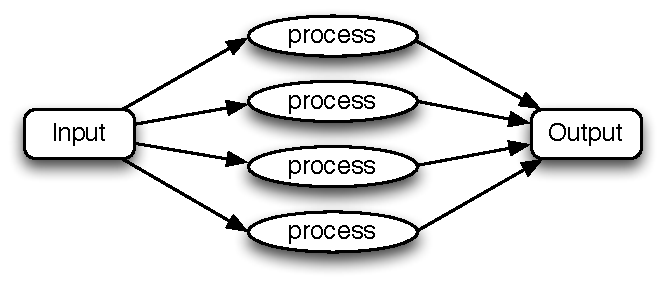
\includegraphics[width=3in]{figs/overview}
  \caption{A high-level architecture of our approach}
  \label{fig:overview}
\end{figure}

% You may need to move this \begin{figure} ... \end{figure} block around
% in the document to place it in a logical spot in the paper. In
% general, get the figure on the same page as the prose that refers to
% it.

